\chapter{Introduction}
\label{chap:introduction}

If someone were to ask you to identify a banking scam within millions of transactions from an ordinary bank account, you would probably think that it should not be too hard. You would just have to develop some kind of computer program that compares the regular transactions made in the past to trace a deviation produced by the scam. But distinguishing this `outlier' by comparing all previous transactions would be very time consuming, also for computers.

In this banking scenario the outliers correspond to all the data points that in some sense significantly deviate from all previously observed, expected or `normal' financial behaviour. However, you are asked to trace those outliers not just for one banking account, but for all of them. And not just once a year or once a month, but continuously! Therefore, the objective of this computer program would be to process all incoming transactions one by one (online) as efficiently and accurately as possible.

You can imagine that detecting outliers is not just useful for the safety of your banking account. It is useful for an endless spectrum of fields, varying from scientific to commercial practices. In the medical field you could think of supporting diagnostic procedures, but it can also be deployed to prevent digital systems from cyber attacks.

The common objective of outlier detection methods is to classify all significantly deviating data points as belonging to the `class' of outliers as good as possible, while classifying all normal data points to the other class. With the use of unsupervised outlier detection methods it is possible to do so without inspecting a large set of historic data first. 
In this thesis, we propose a method that is more efficient than what has been recently proposed.

The following chapter will cover the necessary background information on unsupervised online outlier detection in multivariate time series, and the challenges associated with it.
We also discuss methods developed with the objective to solve this problem, and explain the essence of the method we propose in order to do it more efficiently. Finally, we provide an outline of the remainder of this thesis.


\section{Online outlier detection in multivariate time series}
\label{sec:intro_problemcontext}

When outlier detection methods are deployed to observe a system over time, it is desired to obtain a final decision on the most probable class (outlier or normal) of the incoming data points in real-time. That means that a label should be assigned to each incoming data point preferably before the next one arrives. This is due to the potentially high costs associated with a delayed decision. Outlier detection in real-time is called online outlier detection, but is also known as streaming outlier detection \cite{gupta2014outlier}. 

Within this context, we consider the incoming data stream $\mathbf{X} = {\mathbf{x}_1, \mathbf{x}_{2},...,\mathbf{x}_{n}}$ to exhibit temporal relations between succeeding data points. We focus on these relations explicitly by interpreting the observed feature over time. Such temporal features are called time series, where we refer to multiple time series as multivariate time series. Each $\mathbf{x}_i \in \mathbf{X}$ is then a $d$-dimensional valued vector. Often it is not tractable to keep all data points in memory to use for outlier detection purposes. Hopefully, the assumed relations between successive data points $\mathbf{x}_i$ and $\mathbf{x}_{i+1}$, and among the $d$ time series, enable us to infer a model that describes the overall system behaviour well. However, time series are often characterized by dynamically changing behaviour. This means that we need to learn a model online which, in turn, should adapt well to changes in the dynamics of the time series \cite{ahmad2017unsupervised}.

We define our problem context further as online outlier detection in an unsupervised fashion. Unsupervised detection systems do not require labelled data points in order to be deployed, while supervised methods do. Supervised methods, for example, learn classification rules or parameter settings (referred to as training) from labelled data after which the trained model is deployed on unseen data. For online detection systems it is often simply too time consuming to incorporate such information \cite{ahmad2017unsupervised}. As the structure of the data is unknown on forehand and no manual parameter adaptations can be conducted while the system is running, unsupervised online outlier detection methods are preferred to be not too sensitive to parameters. Yet, most methods are \cite{aggarwal2015outlier}.

Having discussed the primary conditions that constitute our problem context, figure \ref{fig:intro_outlierdetection_process} illustrates the general process of unsupervised online outlier detection in multivariate time series. $O_i$ refers to the output of a method which can be either a discrete label (normal or outlier), or a continuous outlier score indicating the `outlierness' of the input data point $\mathbf{x}_i$.

\begin{figure}[h]
	\centering
	\includegraphics[scale=0.72]{introduction/outlierdetection_process}
	\caption{General process of online outlier detection in multivariate time series.}
	\label{fig:intro_outlierdetection_process}	
	\vspace{-0.1cm}
\end{figure}


\section{The complexity of finding outliers in multivariate time series}
\label{sec:introduction_complexity}

Beside the restrictions of online and unsupervised learning systems, finding outliers in multivariate time series is a challenging task already. 
A first challenge is to have an idea of what should be regarded as an outlier before the respective system is deployed. The behaviour considered normal might change over time, where also outliers might not have been observed before and possibly vary heavily. Besides, what should be regarded as normal behaviour and thus as outliers, depends on the context of the application. In general, finding outliers in time series translates to detecting sudden unexpected changes, hence outliers in time series can be described as (sequences of) data points that exhibit a lack in temporal continuity \cite{aggarwal2015outlier}. 

In general, we can distinguish three categories of outliers: global point outliers, contextual point outliers and collective outliers \cite{chandola2009anomaly}. Global point outliers are characterized by globally deviating values given the remainder of the time series\footnote{Figures \ref{fig:intro_point} to \ref{fig:intro_collective} only show one time series. Yet, we focus on multivariate time series such that $d > 1$.} as shown in figure \ref{fig:intro_point}. Global point outliers can also appear collectively forming a global collective outlier. This type is generally not harder to detect than global point outliers and is therefore not considered separately. 
Outliers as illustrated in figures \ref{fig:intro_contextual} and \ref{fig:intro_collective} are often more difficult to find as their feature values do occur in the remainder of the time series, and are therefore contextual. The difference between these two types is that a collective outlier represents a sequence of data points that should be regarded as an outlier in conjunction, while the value of the time series does not change suddenly. A contextual point outlier is characterized by a sudden and temporary change in feature value.

\vspace{-0.25cm}
\begin{figure}[h]
	\begin{minipage}{0.33\textwidth}
		\centering
		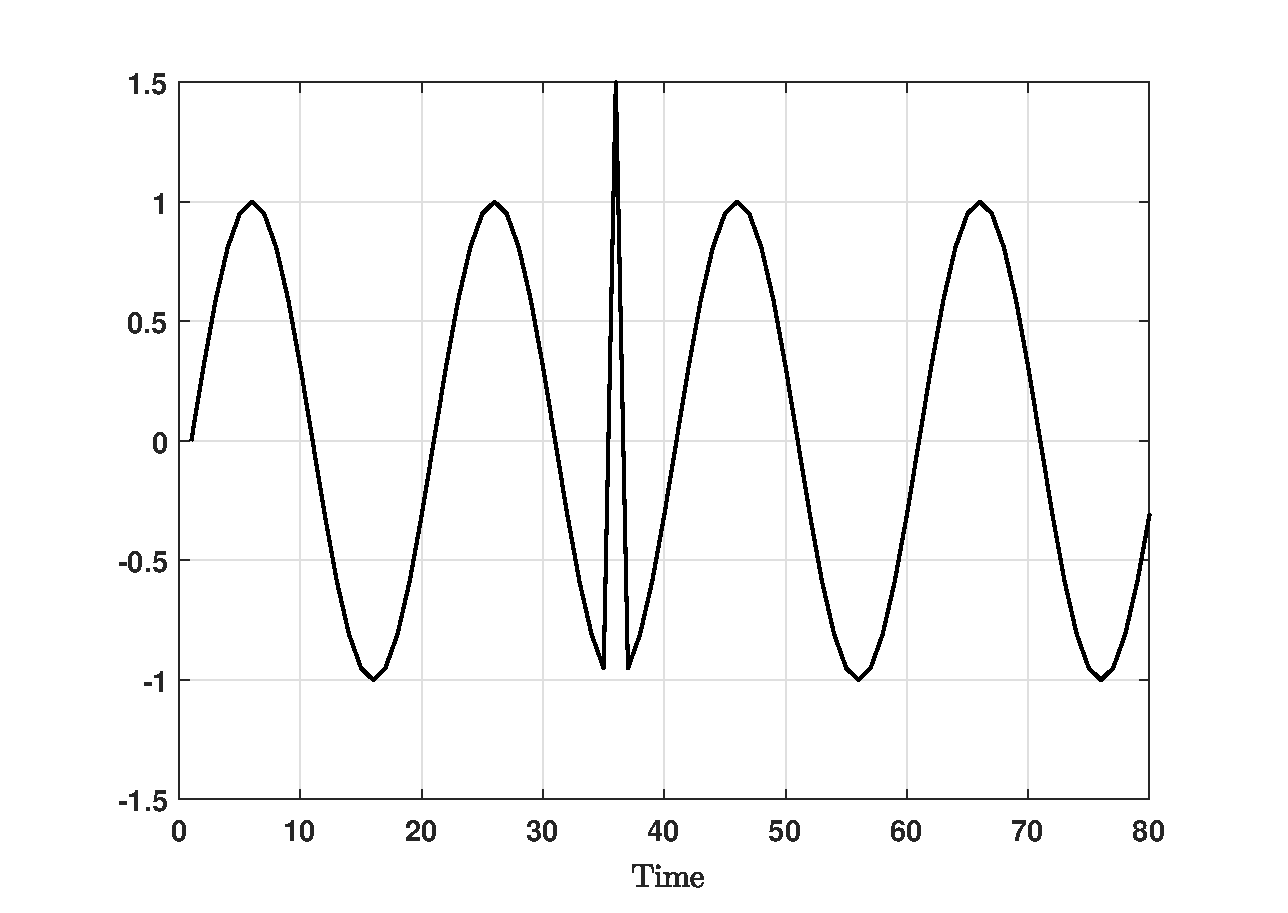
\includegraphics[scale=0.25]{introduction/Point_anomaly}
		\vspace{-0.5cm}
		\caption{Global point outlier.}
		\label{fig:intro_point}
	\end{minipage}
		\vspace{-0.15cm}
	\begin{minipage}{0.33\textwidth}
		\centering
		\includegraphics[scale=0.25]{introduction/Contextual_anomaly}
		\vspace{-0.5cm}
		\hspace{0.15cm}
		\caption{Contextual point outlier.}
		\label{fig:intro_contextual}
	\end{minipage}
		\vspace{-0.15cm}
	\begin{minipage}{0.33\textwidth}
		\centering
		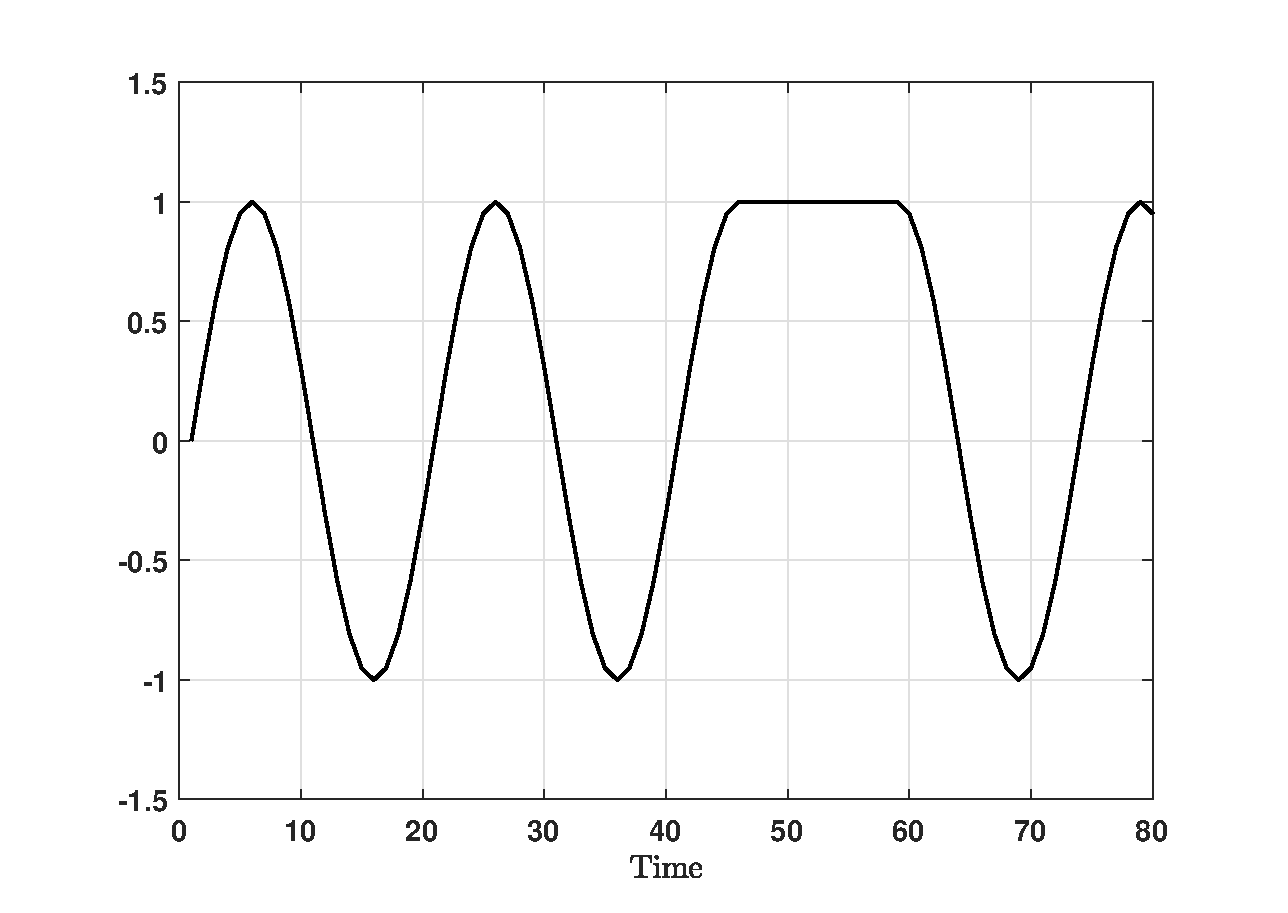
\includegraphics[scale=0.25]{introduction/Collective_anomaly}
		\vspace{-0.5cm}
		\hspace{-0.15cm}
		\caption{Collective outlier.}
		\label{fig:intro_collective}
	\end{minipage}
		\vspace{-0.15cm}
\end{figure}

\newpage
The second challenge associated with outlier detection in multivariate time series is to deal with the effect of the high dimensionality of the data points. Having more features describing each incoming data point might seem to yield a higher chance of observing data points that deviate significantly from what is considered normal. However, having more data at your disposal does not automatically mean that outliers can be separated better from normal data points. At some point, the dimensionality of a data set introduces problems which is often referred to as the curse of dimensionality. 

One problem is that the norms of data points in a data set $\mathbf{X}$ of high dimensionality $d$, for example, tend to approach the same value as the number of features goes to infinity \cite{zimek2012survey}. This means there is little variance between data points in $\mathbf{X}$ if we look at the ratio between the norms of the data points in $\mathbf{X}$ and the norm of the mean of $\mathbf{X}$. As a consequence, the largest distance between a pair of two data points in $\mathbf{X}$ 
approaches the smallest pair-wise distance 
\cite{beyer1999nearest}. This concentration of distances makes the difference between outlier scores associated with outliers and normal data points vanish. 

Another downside is the computational burden induced by processing high-dimensional data points. The main cause of computational issues lies in the search space imposed by an increasing dimensionality. That is, outliers are often characterized by deviating values in a subspace rather than in the full feature space. The consequence is that algorithms often search for meaningful subspaces in which outliers can be discriminated. An increase in the number of features $d$, therefore, implies an exponential growing search space \cite{zimek2012survey}. Going through all $(2^d - 1)$ possible subsets for $d$ features is considered not tractable if $d$ is high.

Table \ref{tab:intro_characteristics} summarizes the challenges associated with each characteristic of outlier detection in multivariate time series in an online and unsupervised manner.

\begin{table}[h]
	\centering
	\caption{Challenges associated with our task.}
	\label{tab:intro_characteristics}
	\begin{tabular}{p{0.3\linewidth} p{0.6\linewidth}}
		\toprule
		\textbf{Characteristic}	&	\textbf{Challenge} \\
		\midrule
		\multirow{8}{*}{Online classification \cite{ahmad2017unsupervised,aggarwal2015outlier}} & The algorithm must assign label $O_i$ to data point ${\mathbf x}_i$ before receiving ${\mathbf x_{i+1}}$.\\[0.12cm]
		& The algorithm should only exploit a limited history of the data to infer its model, and not require storage of the entire stream.\\[0.12cm]
		& The algorithm should run unsupervised, i.e. without the need of labelling data points or manually adapting parameters.\\[0.12cm]
		& The detection performance should be not too sensitive to the (fixed) parameters.\\
		\midrule 
		\multirow{3}{*}{Outlier detection in} & The analyst should have an idea of the expected, normal behaviour, and of the outliers desired to detect. \\[0.12cm]
		time series \cite{chandola2009anomaly}& The algorithm should be able to detect contextual outliers besides global outliers. \\
		\midrule
		\multirow{4}{*}{High-dimensional data \cite{zimek2012survey}} & The algorithm should be able to find outliers in high-dimensional data. \\[0.12cm]
		& Algorithms should scale well in computational complexity with increasing numbers of time series $d$ and data points $n$.\\
		\bottomrule
	\end{tabular}
\end{table}



\section{Unsupervised online methods}

As a consequence of the diverse challenges as described, many approaches to unsupervised online outlier detection in multivariate time series exist. In this section we discuss a few recently proposed methods, which can be categorized in proximity-based and model-based methods. The application considered and the outliers expected, often make a certain method more suitable than others. For a discussion of existing methods in relation to common applications of online outlier detection in time series we refer to the surveys by Gupta et al. \cite{gupta2014outlier} and Chandola et al. \cite{chandola2009anomaly}. 

\subsection{Related methods}
\label{sec:introduction_related}
Proximity-based methods examine the spatial proximity of data points to discriminate data points that significantly deviate from the proximity of the majority of data points. The proximity of an incoming data point is mostly reflected by a distance or density measure in context of its preceding data points.
A recently developed density-based method is Loda, short for light-weight online detector of anomalies\footnote{The term \textit{anomalies} is considered to refer to the same concept as \textit{outliers}.} \cite{pevny2016loda}. Loda projects the incoming data point into $k$ random $1$-dimensional subspaces and maintains $k$ histograms with $b$ bins to approximate a probability density function. The average of the log probability approximated by these $k$ histograms, is assigned to the data point as its outlier score. The histograms are constantly updated as new data points come in. 

A distance-based method suitable for online outlier detection in high-dimensional data streams is LEAP \cite{cao2014scalable}. LEAP slides a window of size $p$ over the data stream and computes the distance of an incoming data point $\mathbf{x}_i$ to data points within this window. It does so until there is minimal yet enough evidence that $\mathbf{x}_i$ is not an outlier. If the minimal evidence threshold is not exceeded, the entire neighbourhood of the data point is evaluated. This minimal evidence threshold is based on the distance between the incoming data point and a few prototype data points in its surrounding window. Such prototypes are selected over time, which implies that the total reference set evolves over time. A data point is flagged as an outlier if its distance to the prototypes, or to all data points in the current window exceed a threshold.

\vspace{0.1cm}

Model-based outlier detection methods describe the expected behaviour of the multivariate time series with a model. Various options exist for modelling the data online and use the resulting model to generate binary labels or outlier scores for incoming data points. Recently, Ahmad et al. \cite{ahmad2017unsupervised} proposed an unsupervised method that models the data online using Hierarchical Temporal Memory (HTM) networks. Such networks encode data points in a lower-dimensional subspace and represent it as a sparse binary vector. A so-called sequence memory component models the temporal patterns from these binary vectors and generates predictions for upcoming data points. A more detailed explanation of HTM networks can be found in \cite{cui2016continuous}. Ahmad et al. use this technique to infer outlier scores from the distribution of historic prediction errors generated by the HTM network.

A different model-based approach, principal component analysis (PCA), also represents the $d$ time series in a lower-dimensional subspace. It does so by linearly projecting the data into directions in which most of the variance in the data is captured \cite{jolliffe1986principal}. After projecting the data into this optimized subspace, the lower-dimensional representation is reconstructed to the original dimensionality $d$. The outliers are then hopefully not explained by the principal components, such that the distance between the original data points and their reconstructions yields a discriminative outlier measure. A well-known method to approximate the principal components unsupervised and online is SPIRIT \cite{papadimitriou2005streaming}. SPIRIT is considered to be a tractable and effective method for online outlier detection in multivariate time series \cite{aggarwal2015outlier}. As it has strong similarities with the method we propose, we explain this method in more detail in chapter \ref{chap:reconstruction-detection}. 

The methods discussed in this section are suitable for unsupervised online outlier detection in multivariate time series and considerably effective. Still, we think there is a promising direction left unexplored that introduces methods to solve this problem in a more efficient manner.


\subsection{The proposed method in a nutshell}
In this thesis we attempt to address the challenges as listed in table \ref{tab:intro_characteristics} with only one method: random projections. The proposed random projection method projects or maps data points of high dimensionality $d$ into a random $k$-dimensional subspace. If our mapping function $\mathbf{f}$ satisfies certain conditions, we are guaranteed that the obtained lower dimensional representation preserves the pair-wise Euclidean distances in our data stream ${\mathbf X}$ up to some error \cite{johnson1984extensions}. The obtained $k$-dimensional representation of a data point at time step $i$, $\mathbf{x}_i'$, is reconstructed back into the original dimensionality $d$. This reconstructed data point $\hat{\mathbf{x}}_i$ then functions as a model of the original data point $\mathbf{x}_i$. As this method does not update any projection directions or optimize mapping functions on the data, it is an efficient method.

The first proposed use of this method interprets the squared Euclidean distance between $\mathbf{x}_i$ and $\hat{\mathbf{x}}_i$ as the outlier score $O_i$ as in equation \eqref{eq:intro_squared_euclidean}. 

\begin{equation}\label{eq:intro_squared_euclidean}
	O_i =\left( \ \sqrt{\sum\limits_{j=1}^d (\mathbf{x}_{i,j} - \hat{\mathbf{x}}_{i,j})^2} \ \right)^2 = \sum\limits_{j=1}^d (\mathbf{x}_{i,j} - \hat{\mathbf{x}}_{i,j})^2
\end{equation}

\noindent Throughout the remainder of this thesis we represent this distance as $\|\mathbf{x}_i - \hat{\mathbf{x}}_i\|^2$. The conversion from this continuous score to a discrete label is considered beyond the scope of this thesis as the level of outlierness corresponding to an `actual' outlier likely depends on the system being observed.


Contextual outliers are particularly hard to detect with our method using this outlier measure. Therefore, we present an additional interpretation of the reconstructions obtained from random projections that enables detecting contextual outliers as well. This alternative is based on $2$ distinct runs of the random projection method with different values for the number of projection vectors $k$. We take the difference between the two obtained reconstructions as indicator of the outlierness at time step $i$. This method is explained in more detail in chapter \ref{chap:analysis}.

Projecting the data into random directions implies the projection is not optimized on the data at hand, and is therefore called data-independent. Beside its benefits for the runtime performance, a data-independent method also makes theoretical analysis of its properties possible. For example, the lower bound on the projection dimensionality $k$ only depends on the number of data points $n$, the choice for random mapping $\mathbf{f}$ and maximum distortion $\varepsilon$. This enables full control over the quality of the lower-dimensional representation as we can choose $\mathbf{f}$ and an acceptable distortion $\varepsilon$. In chapter \ref{chap:rp-method} we thoroughly explain the random projection method.

The question we focus on throughout this thesis is: \textit{can we leverage random projections in an online and unsupervised reconstruction-based method in order to find outliers in multivariate time series effectively though more efficiently, and if so, to what extent?} 
In particular, we investigate if and to what extent the method we propose defeats the challenges as summarized in table \ref{tab:intro_characteristics}.


\section{Outline of this thesis}

In this chapter, we have formulated the problem context and explained the challenges it imposes. We also provided an overview of related methods to conduct online outlier detection in multivariate time series, and briefly explained the proposed method. The remainder of this thesis is organized as follows. First, we explain the general approach of reconstruction-based outlier detection in more detail in chapter \ref{chap:reconstruction-detection}. We proceed in chapter \ref{chap:rp-method} with the formulation of the proposed random projection method. An analysis of this method on synthetic data follows in chapter \ref{chap:analysis}. Chapter \ref{chap:experiments} presents the results of experiments conducted with real-world time series data, where we also explore the applicability of the random projection method on non-temporal data sets. We conclude this thesis in chapter \ref{chap:discussion} with an overview of the key findings and conclusions, and suggestions for future work.


